\documentclass[12pt,a4paper]{article}

% ─── Page Layout ───────────────────────────────────────────────────────────────
\usepackage[a4paper, margin=0.8in, headheight=14pt]{geometry}

% ─── Fonts (XeLaTeX) ───────────────────────────────────────────────────────────
\usepackage{fontspec}
\usepackage{unicode-math}
\setmainfont{TeX Gyre Pagella}
\setmonofont[Scale=0.88]{TeX Gyre Cursor}
\setmathfont{Latin Modern Math}

% ─── Packages ──────────────────────────────────────────────────────────────────
\usepackage{xcolor}
\usepackage{colortbl}
\usepackage{titlesec}
\usepackage{enumitem}
\usepackage{tabularx}
\usepackage{booktabs}
\usepackage{array}
\usepackage{amsmath}
\usepackage{tikz}
\usetikzlibrary{shapes.geometric, arrows.meta, positioning, calc, fit, decorations.pathreplacing}
\usepackage{tcolorbox}
\tcbuselibrary{skins, breakable}
\usepackage{hyperref}
\usepackage{fancyhdr}
\usepackage{graphicx}
\usepackage{microtype}
\hyphenpenalty=10000
\exhyphenpenalty=10000
\sloppy
\usepackage{caption}
\usepackage{setspace}
\usepackage{multirow}
\usepackage{tocloft}

% ─── Q&A helper ────────────────────────────────────────────────────────────────
\newcommand{\Q}[1]{\textbf{#1}\par\noindent\ignorespaces}

% ─── Colour Palette ────────────────────────────────────────────────────────────
\definecolor{myred}{RGB}{196,30,58}
\definecolor{mydark}{RGB}{30,30,50}
\definecolor{mygreen}{RGB}{14,120,80}
\definecolor{myteal}{RGB}{0,130,140}
\definecolor{myamber}{RGB}{180,100,0}
\definecolor{mypurple}{RGB}{100,30,160}
\definecolor{mygray}{RGB}{246,247,249}
\definecolor{mgframe}{RGB}{180,185,200}
\definecolor{watermark}{RGB}{145,150,170}
\definecolor{hdrred}{RGB}{250,232,235}
\definecolor{hdrgreen}{RGB}{220,244,233}
\definecolor{hdrteal}{RGB}{220,242,244}
\definecolor{hdramber}{RGB}{253,242,215}
\definecolor{hdrpurple}{RGB}{238,228,255}
\definecolor{hdrgray}{RGB}{238,240,245}
\definecolor{rowalt}{RGB}{250,251,253}

% ─── Section Formatting ────────────────────────────────────────────────────────
\titleformat{\section}
  {\large\bfseries\color{myred}}{\thesection.}{0.5em}{}
  [\vspace{1pt}{\color{myred}\rule{\linewidth}{0.8pt}}]
\titleformat{\subsection}
  {\normalsize\bfseries\color{myteal}}{\thesubsection}{0.5em}{}
\titlespacing*{\section}{0pt}{18pt}{7pt}
\titlespacing*{\subsection}{0pt}{11pt}{4pt}

% ─── Paragraph ─────────────────────────────────────────────────────────────────
\setlength{\parindent}{0pt}
\setlength{\parskip}{4pt}

% ─── TOC Styling ───────────────────────────────────────────────────────────────
\renewcommand{\cfttoctitlefont}{\large\bfseries\color{myred}}
\renewcommand{\cftaftertoctitle}{\par\noindent{\color{myred}\rule{\linewidth}{0.8pt}}}
\setlength{\cftbeforetoctitleskip}{0pt}
\setlength{\cftaftertoctitleskip}{6pt}
\renewcommand{\cftsecfont}{\normalsize\bfseries\color{mydark}}
\renewcommand{\cftsecpagefont}{\normalsize\bfseries\color{mydark}}
\renewcommand{\cftsecleader}{\cftdotfill{\cftdotsep}}
\setlength{\cftbeforesecskip}{7pt}
\renewcommand{\cftsubsecfont}{\small\color{mydark}}
\renewcommand{\cftsubsecpagefont}{\small\color{mydark}}
\setlength{\cftbeforesubsecskip}{3pt}
\setlength{\cftsubsecindent}{1.4em}

% ─── Table helpers ─────────────────────────────────────────────────────────────
\renewcommand{\arraystretch}{1.45}
\setlength{\tabcolsep}{6pt}
\arrayrulecolor{mydark}
\newcolumntype{B}[1]{>{\small\bfseries\raggedright\arraybackslash}m{#1}}
\newcolumntype{C}[1]{>{\centering\arraybackslash}m{#1}}
\newcolumntype{Y}{>{\small\raggedright\arraybackslash}X}
\renewcommand{\tabularxcolumn}[1]{m{#1}}

% ─── Header / Footer ───────────────────────────────────────────────────────────
\pagestyle{fancy}
\fancyhf{}
\fancyhead[L]{\small\color{myred}\textbf{OE-EC803C}\;\color{mydark}--- Cyber Security}
\fancyhead[R]{\small\color{myteal}\textbf{Module 1 Notes}}
\fancyfoot[C]{\small\color{mydark}\thepage}
\fancyfoot[R]{\small\color{watermark}\textit{\copyright\ Biraj Sarkar}}
\renewcommand{\headrulewidth}{0.5pt}
\renewcommand{\footrulewidth}{0.3pt}

% ─── Hyperref ──────────────────────────────────────────────────────────────────
\hypersetup{
  colorlinks=true, linkcolor=myteal, urlcolor=myteal,
  pdfauthor={Biraj Sarkar},
  pdftitle={OE-EC803C --- Module 1 Notes}
}

% ─── tcolorbox styles ──────────────────────────────────────────────────────────
\tcbset{
  tikzbox/.style={
    colback=mygray, colframe=mgframe, boxrule=0.6pt, arc=4pt,
    left=8pt, right=8pt, top=6pt, bottom=6pt,
    colbacktitle=mgframe, coltitle=mydark,
    fonttitle=\small\bfseries
  },
  defbox/.style={
    colback=hdrgreen, colframe=mygreen, boxrule=0.8pt, arc=4pt,
    left=9pt, right=9pt, top=6pt, bottom=6pt,
    colbacktitle=mygreen, coltitle=white,
    fonttitle=\small\bfseries
  },
  formulabox/.style={
    colback=hdrteal, colframe=myteal, boxrule=0.8pt, arc=4pt,
    left=9pt, right=9pt, top=7pt, bottom=7pt,
    colbacktitle=myteal, coltitle=white,
    fonttitle=\small\bfseries
  },
  examplebox/.style={
    colback=hdramber, colframe=myamber, boxrule=0.8pt, arc=4pt,
    left=9pt, right=9pt, top=6pt, bottom=6pt,
    colbacktitle=myamber, coltitle=white,
    fonttitle=\small\bfseries
  },
  masonbox/.style={
    colback=hdrpurple, colframe=mypurple, boxrule=0.8pt, arc=4pt,
    left=9pt, right=9pt, top=6pt, bottom=6pt,
    colbacktitle=mypurple, coltitle=white,
    fonttitle=\small\bfseries
  },
  exambox/.style={
    colback=hdrpurple, colframe=mypurple, boxrule=1pt, arc=5pt,
    left=10pt, right=10pt, top=8pt, bottom=8pt,
    colbacktitle=mypurple, coltitle=white, fonttitle=\bfseries,
    breakable, title after break={\textbf{Frequently Asked / Viva Questions (contd.)}}
  }
}
\tcbset{breakable}

% ─── TikZ styles ───────────────────────────────────────────────────────────────
\tikzset{
  block/.style={rectangle, draw=myteal, fill=hdrteal,
    text width=2.2cm, align=center, minimum height=0.9cm,
    font=\small, rounded corners=3pt, line width=0.7pt},
  redblock/.style={rectangle, draw=myred, fill=hdrred,
    text width=2.2cm, align=center, minimum height=0.9cm,
    font=\small, rounded corners=3pt, line width=0.7pt},
  arrow/.style={-Stealth, thick, color=mydark},
  redarrow/.style={-Stealth, thick, color=myred},
  line/.style={thick, color=mydark}
}

\begin{document}

% ═══════════════════════════════════════════════════════════════════════════════
% TITLE BLOCK
% ═══════════════════════════════════════════════════════════════════════════════
\begin{center}
  \hfill \textit{Exam-Ready Short Notes} \\
  \vspace{6pt}
  {\LARGE\bfseries\color{myred} OE-EC803C --- Cyber Security}\\[5pt]
  {\normalsize\color{mydark} Semester VIII \quad$\bullet$\quad 3L:0T:0P \quad$\bullet$\quad 3 Credits}\\[3pt]
  {\normalsize\color{myteal}\textbf{Module 1: Introduction to Cyber Security \& Policy}}\\[3pt]
  {\small\color{mydark} CGEC \;$|$\; B.Tech ECE (2023--27) \;$|$\; \textit{Biraj Sarkar}}
\end{center}
\vspace{2pt}
\noindent{\color{myred}\rule{\linewidth}{1.5pt}}
\vspace{2pt}

\hypersetup{linkcolor=mydark}
\tableofcontents
\hypersetup{linkcolor=myteal}
\newpage

% ===============================================================================
\section{Cyber Security Fundamentals \& Evolution}
% ===============================================================================

Cyber Security encompasses the technologies, processes, and governance policies designed to protect networks, computer devices, software applications, and critical data from unauthorized access, cyber attacks, or service disruption.

\begin{tcolorbox}[defbox, title={\textbf{Definition: The CIA Triad \& Parkerian Hexad}}]
\begin{itemize}[leftmargin=*, itemsep=3pt]
  \item \textbf{Confidentiality:} Ensuring data is accessible only to authorized entities. Enforced via AES-256 encryption, access control lists (ACLs), and TLS protocols.
  \item \textbf{Integrity:} Protecting data accuracy against unauthorized modification or tampering. Enforced via SHA-256 cryptographic hashes and digital signatures.
  \item \textbf{Availability:} Guaranteeing timely, uninterrupted system access for authorized users. Enforced via redundant hardware, load balancing, and DDoS mitigations.
  \item \textbf{Parkerian Hexad Extensions:} Extends CIA triad by adding \textit{Authenticity} (verifying identity), \textit{Utility} (usefulness of data), and \textit{Possession/Control} (physical/logical custody).
\end{itemize}
\end{tcolorbox}

\subsection{Generational Evolution of Cyber Threats}
Cyber threat vectors have evolved over four distinct historical eras:
\begin{enumerate}[leftmargin=*, itemsep=4pt]
  \item \textbf{First Generation (1980s--1990s):} Standalone boot-sector viruses and early worms (Brain Virus, Morris Worm) transmitted via floppy disks. Defense relied on signature-based antivirus scanning.
  \item \textbf{Second Generation (2000s):} Network-propagating worms and mass-mailing malware (ILOVEYOU, Code Red, Slammer). Introduced stateful firewalls and Intrusion Detection Systems (IDS).
  \item \textbf{Third Generation (2010s):} Advanced Persistent Threats (APTs), polymorphic ransomware (WannaCry, NotPetya), and distributed botnets. Introduced Next-Generation Firewalls (NGFW) and Endpoint Detection \& Response (EDR).
  \item \textbf{Fourth Generation (2020s--Present):} AI-driven deepfake social engineering, zero-day supply chain breaches (SolarWinds), and cloud-native infrastructure targeted attacks.
\end{enumerate}

\subsection{Defense-in-Depth Architecture}
Defense-in-Depth enforces multiple layered security controls across the enterprise:

\begin{tcolorbox}[tikzbox, title={Defense-in-Depth Layered Model}]
\centering
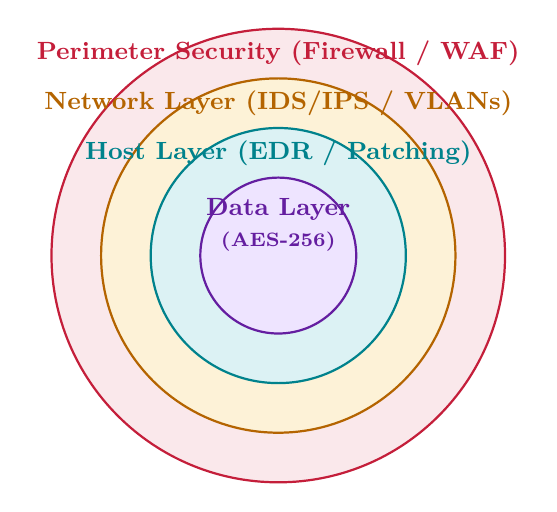
\begin{tikzpicture}[scale=0.9]
  \draw[fill=hdrred, draw=myred, line width=0.8pt] (0,0) circle (3.2cm);
  \draw[fill=hdramber, draw=myamber, line width=0.8pt] (0,0) circle (2.5cm);
  \draw[fill=hdrteal, draw=myteal, line width=0.8pt] (0,0) circle (1.8cm);
  \draw[fill=hdrpurple, draw=mypurple, line width=0.8pt] (0,0) circle (1.1cm);

  \node[font=\small\bfseries\color{myred}] at (0,2.85) {Perimeter Security (Firewall / WAF)};
  \node[font=\small\bfseries\color{myamber}] at (0,2.15) {Network Layer (IDS/IPS / VLANs)};
  \node[font=\small\bfseries\color{myteal}] at (0,1.45) {Host Layer (EDR / Patching)};
  \node[font=\small\bfseries\color{mypurple}] at (0,0.65) {Data Layer};
  \node[font=\scriptsize\bfseries\color{mypurple}] at (0,0.2) {(AES-256)};
\end{tikzpicture}
\end{tcolorbox}

% ===============================================================================
\section{Cyber Security Policy \& Governance Domains}
% ===============================================================================

\begin{tcolorbox}[defbox, title={\textbf{Definition: Security Policy Hierarchy}}]
A \textbf{Security Policy} defines mandatory rules establishing governance boundaries. Governance follows a strict three-tier hierarchy:
\end{tcolorbox}

{\renewcommand{\arraystretch}{1.45}%
\begin{tabularx}{\linewidth}{|B{3.0cm}|Y|Y|}
\hline
\textbf{Governance Tier} & \textbf{Primary Objective} & \textbf{Audience \& Enforcement} \\
\hline
Strategy & Defines long-term cybersecurity vision, risk posture, and 3-to-5 year strategic roadmaps. & Executive Board, CISO, CIO. \\
\hline
Policy & Establishes mandatory compliance rules, responsibilities, and operational boundaries. & All Employees, Contractors, System Admins. \\
\hline
Procedure & Standard Operating Procedures (SOPs) detailing step-by-step technical execution. & IT Operations, Security Engineers, Helpdesk. \\
\hline
\end{tabularx}}

\subsection{Key Operational Policy Domains}
\begin{itemize}[leftmargin=*, itemsep=3pt]
  \item \textbf{Acceptable Use Policy (AUP):} Specifies acceptable employee behavior regarding corporate hardware, internet browsing, and email usage.
  \item \textbf{Access Control Policy:} Enforces Role-Based Access Control (RBAC), Multi-Factor Authentication (MFA), and the Principle of Least Privilege.
  \item \textbf{Data Classification Policy:} Categorizes data into Public, Internal, Confidential, and Restricted tiers to determine required encryption controls.
  \item \textbf{Incident Response Policy:} Outlines 6-phase incident response steps: Preparation $\to$ Identification $\to$ Containment $\to$ Eradication $\to$ Recovery $\to$ Lessons Learned.
\end{itemize}

% ===============================================================================
\section{Laws, Regulations \& Regulatory Compliance}
% ===============================================================================

Cyber policy must align strictly with statutory legal frameworks:

\begin{tcolorbox}[defbox, title={\textbf{Detailed Indian IT Act 2000 Section Breakdown}}]
\begin{itemize}[leftmargin=*, itemsep=3pt]
  \item \textbf{Section 43:} Penalty for damaging computer systems, unauthorized downloading, or introducing virus contaminants (fine up to INR 1 Crore).
  \item \textbf{Section 65:} Punishment for tampering with computer source documents (imprisonment up to 3 years or fine up to INR 2 Lakhs).
  \item \textbf{Section 66:} Hacking with computer system (dishonestly or fraudulently damaging system data).
  \item \textbf{Section 66B / 66C / 66D:} Punishment for receiving stolen computer resource, identity theft, and cheating by impersonation using computer resources.
  \item \textbf{Section 66E / 66F:} Punishment for capturing/publishing private images without consent, and \textbf{Cyber Terrorism} (denying access to critical national infrastructure with intent to threaten national unity; penalty: \textbf{Life Imprisonment}).
  \item \textbf{Section 79:} Intermediary liability safe-harbor guidelines requiring platforms (e.g. social media) to observe due diligence.
\end{itemize}
\end{tcolorbox}

% ===============================================================================
\section{Technology Operations and System Hardening}
% ===============================================================================

System hardening reduces an asset's attack surface by eliminating default security weaknesses:

\begin{enumerate}[leftmargin=*, itemsep=4pt]
  \item \textbf{Disabling Default Credentials \& Unused Ports:} Changing default administrative passwords (e.g. `admin/admin`) and closing unnecessary open ports (e.g. disabling Telnet port 23 in favor of SSH port 22).
  \item \textbf{Automated Patch Management:} Deploying centralized patch management (e.g. WSUS) to test and push vendor security updates within strict SLAs.
  \item \textbf{Configuration Baselining:} Utilizing Center for Internet Security (CIS) Benchmarks to lock down OS configurations via Group Policy Objects (GPO).
\end{enumerate}

% ===============================================================================
\section{Botnets, DDoS Attacks \& Case Studies}
% ===============================================================================

A \textbf{Botnet} is a network of compromised internet-connected devices (bots) controlled remotely by a Botmaster via a Command and Control (C2) server.

\begin{tcolorbox}[tikzbox, title={Botnet Command and Control (C2) Flow}]
\centering
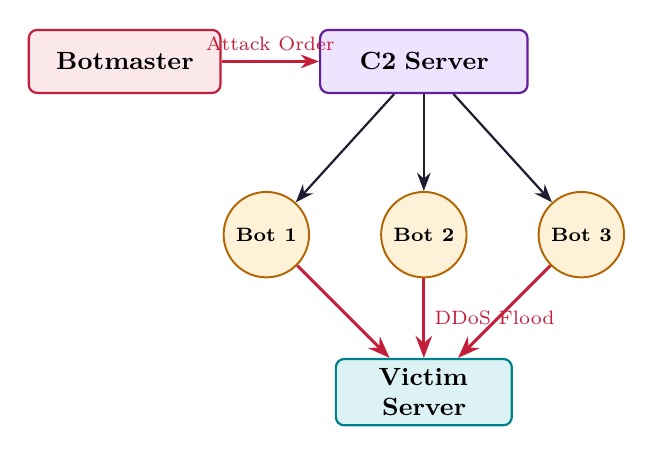
\begin{tikzpicture}[node distance=1.2cm and 1.5cm,
  bm/.style={rectangle, draw=myred, fill=hdrred, text width=2.2cm, align=center, minimum height=0.8cm, font=\small\bfseries, rounded corners=3pt, line width=0.8pt},
  c2/.style={rectangle, draw=mypurple, fill=hdrpurple, text width=2.4cm, align=center, minimum height=0.8cm, font=\small\bfseries, rounded corners=3pt, line width=0.8pt},
  bot/.style={circle, draw=myamber, fill=hdramber, align=center, minimum size=0.75cm, font=\scriptsize\bfseries, line width=0.7pt},
  tgt/.style={rectangle, draw=myteal, fill=hdrteal, text width=2.0cm, align=center, minimum height=0.8cm, font=\small\bfseries, rounded corners=3pt, line width=0.8pt},
  arrow/.style={-Stealth, thick, color=mydark},
  redarrow/.style={-Stealth, thick, color=myred}]

  \node[bm] (b1) at (0,2.2) {Botmaster};
  \node[c2] (c1) at (3.8,2.2) {C2 Server};
  \node[bot] (z1) at (1.8,0) {Bot 1};
  \node[bot] (z2) at (3.8,0) {Bot 2};
  \node[bot] (z3) at (5.8,0) {Bot 3};
  \node[tgt] (v1) at (3.8,-2.0) {Victim Server};

  \draw[redarrow] (b1) -- node[above, font=\scriptsize] {Attack Order} (c1);
  \draw[arrow] (c1) -- (z1);
  \draw[arrow] (c1) -- (z2);
  \draw[arrow] (c1) -- (z3);
  \draw[redarrow, line width=1.1pt] (z1) -- (v1);
  \draw[redarrow, line width=1.1pt] (z2) -- node[right, font=\scriptsize] {DDoS Flood} (v1);
  \draw[redarrow, line width=1.1pt] (z3) -- (v1);

\end{tikzpicture}
\end{tcolorbox}

\begin{tcolorbox}[examplebox, title={\textbf{Real-World Case Study: Mirai Botnet Attack (2016)}}]
\begin{enumerate}[leftmargin=*, itemsep=3pt]
  \item \textbf{Infection Vector:} Mirai scanned the public internet for vulnerable IoT devices (CCTV cameras, home routers) protected only by 60 factory default username/password combinations.
  \item \textbf{Execution:} Infected over 600,000 IoT devices, building a massive distributed botnet without user knowledge.
  \item \textbf{Impact:} Executed a record-breaking $1.2\text{ Tbps}$ DNS SYN flood against Dyn DNS provider, knocking offline major platforms including Twitter, Netflix, Reddit, and Spotify across the US East Coast.
\end{enumerate}
\end{tcolorbox}

% ═══════════════════════════════════════════════════════════════════════════════
% QUICK REVISION PAGE
% ═══════════════════════════════════════════════════════════════════════════════
\newpage
\begin{center}
  {\large\bfseries\color{myred} Quick Revision --- Module 1}\\[3pt]
  {\small\color{mydark} Introduction to Cyber Security \& Policy $|$ OE-EC803C}
\end{center}
\noindent{\color{myred}\rule{\linewidth}{1.2pt}}
\vspace{4pt}

\begin{tcolorbox}[formulabox, title={\textbf{Key Concepts and Metrics at a Glance}}]
\renewcommand{\arraystretch}{1.35}
\begin{tabularx}{\linewidth}{B{4.5cm} X}
CIA Triad & Confidentiality (AES), Integrity (SHA-256), Availability (Redundancy/DDoS defense). \\[3pt]
Section 66F IT Act & Indian cyber law prescribing Life Imprisonment for Cyber Terrorism. \\[3pt]
Mirai Botnet & IoT botnet exploit utilizing default credentials to generate $1.2\text{ Tbps}$ DDoS attacks. \\[3pt]
Defense-in-Depth & Multi-layered security (Perimeter $\to$ Network $\to$ Host $\to$ Application $\to$ Data). \\[3pt]
AUP Policy & Acceptable Use Policy governing permissible workplace IT resource usage.
\end{tabularx}
\end{tcolorbox}

\begin{tcolorbox}[defbox, title={\textbf{One-Line Definitions}}]
\begin{itemize}[leftmargin=*, itemsep=2pt, topsep=0pt]
  \item \textbf{System Hardening:} Disabling unnecessary services and ports to minimize vulnerability attack surface.
  \item \textbf{C2 Server:} Centralized command server used by botmasters to send instructions to infected bots.
  \item \textbf{Parkerian Hexad:} Security model expanding CIA with Authenticity, Utility, and Possession.
  \item \textbf{Intermediary Safe Harbor:} Legal protection for web platforms under Section 79 of Indian IT Act.
\end{itemize}
\end{tcolorbox}

\begin{tcolorbox}[exambox, title={\textbf{Frequently Asked / Viva Questions}}]
\begin{enumerate}[leftmargin=*, label=\textbf{Q\arabic*.}, itemsep=5pt, topsep=0pt]
  \item \Q{Define the CIA Triad and give one technical control for each pillar.}
        Confidentiality (AES-256 encryption), Integrity (SHA-256 hashing), Availability (load balancing and DDoS mitigations).

  \item \Q{Differentiate between a Security Policy, Strategy, and Procedure.}
        Strategy is executive vision; Policy is mandatory compliance rules; Procedure is step-by-step technical execution instructions.

  \item \Q{What penalty does Section 66F of the Indian IT Act 2000 impose?}
        Life imprisonment for committing Cyber Terrorism against critical national infrastructure.

  \item \Q{Explain the architecture of a Botnet Command and Control (C2) server.}
        The botmaster issues commands to the centralized C2 server, which relays orders to thousands of infected zombie bots to execute attacks.

  \item \Q{What is System Hardening and why is it important?}
        The process of locking down OS configurations, disabling unused ports/services, and applying security patches to minimize attack surface.

  \item \Q{Describe the Mirai Botnet case study of 2016.}
        Mirai compromised 600,000+ IoT devices using factory default passwords, generating a $1.2\text{ Tbps}$ DDoS attack that knocked Dyn DNS offline.

  \item \Q{What is an Acceptable Use Policy (AUP)?}
        A mandatory document defining acceptable and prohibited employee activities on corporate networks, laptops, and internet channels.

  \item \Q{Explain the Defense-in-Depth security model.}
        Deploying multiple redundant security layers (firewall, network IDS, host EDR, data encryption) so if one layer fails, subsequent layers block the attack.

  \item \Q{What is Section 43 of the Indian IT Act?}
        Imposes civil liability and damages up to INR 1 Crore for unauthorized system access, downloading data, or inserting malware.

  \item \Q{What are the 6 phases of Incident Response?}
        Preparation $\to$ Identification $\to$ Containment $\to$ Eradication $\to$ Recovery $\to$ Lessons Learned.

  \item \Q{Explain the Parkerian Hexad framework.}
        An expanded security framework adding Authenticity, Utility, and Possession/Control to the traditional CIA triad.

  \item \Q{Why is attribution difficult in cyber crime investigations?}
        Attackers route malicious traffic through encrypted Tor nodes, VPN proxies, and spoofed IP headers across multi-national jurisdictions.

  \item \Q{What is the Principle of Least Privilege?}
        Granting users and service accounts only the minimum access rights needed to perform their assigned work tasks.

  \item \Q{Explain the threat of Fourth-Generation cyber attacks.}
        AI-driven deepfake phishing, automated zero-day exploit discovery, and targeted supply chain software breaches.

  \item \Q{What is Section 79 of the Indian IT Act?}
        Provides safe-harbor immunity to network intermediaries (ISPs, social media platforms) if they observe government due diligence.
\end{enumerate}
\end{tcolorbox}

\begin{tcolorbox}[tikzbox, title={Summary Comparison: Cyber Security Governance Tiers}]
\centering
{\renewcommand{\arraystretch}{1.45}%
\begin{tabularx}{\linewidth}{|B{2.8cm}|Y|Y|Y|}
\hline
\textbf{Governance Tier} & \textbf{Mandatory Level} & \textbf{Focus Area} & \textbf{Revision Cycle} \\
\hline
Strategy & Visionary & Business Alignment & 3 to 5 Years \\
\hline
Policy & Mandatory & Governance Rules & Annual Review \\
\hline
Procedure & Mandatory & Technical Steps & Continuous / Quarterly \\
\hline
Guideline & Optional & Best Practice Advice & As Needed \\
\hline
\end{tabularx}}
\end{tcolorbox}

\end{document}
